% ============================================================
%  N.2  Single-Architecture Experiment Results
% ============================================================
\section{Single-Architecture Sensitivity Analysis}
\label{sec:single-arch}

This section presents sensitivity sweeps performed on each architecture
in isolation, varying one design parameter at a time while keeping all
others fixed.
The goal is to understand how tile size, PE array dimensions, and
register sizing affect energy, latency, and EDP for each workload
before moving to the fusion comparison in Section~\ref{sec:fusion}.

% ============================================================
%  N.2.1  DepFiN CS1: Tile Size Sweep
% ============================================================
\subsection{DepFiN: Tile Size Sensitivity (CS1)}
\label{sec:cs1-tile}

\subsubsection{Motivation}

In the DepFiN-Like architecture the output tile size determines how
many output columns are computed in parallel across the PE array
columns.
A tile of width~$t$ occupies $t$~of the 128 available columns, so
the number of temporal passes over the output spatial
dimension~$Q$ at the DRAM level is $\lceil Q / t \rceil$.
Reducing the tile size therefore multiplies the number of DRAM-level
iterations, which has two consequences:
%
\begin{enumerate}
  \item \textbf{Latency increases} almost linearly, because
        each additional pass requires a full traversal of all
        fused layers for that tile slice.
  \item \textbf{Weight re-reads increase}: at every new tile pass the
        entire weight set must be re-fetched from the Weight Memory (WMEM)
        into the per-PE weight registers, since the weights must be available for each pass.
\end{enumerate}
%
The Feature Memory (FMEM) read bandwidth is scaled proportionally to the tile size
($\text{BW}_{\text{scaled}} = \text{BW}_{\text{base}} \times t / 128$) to reflect the reduced wordline utilization at smaller tiles,
without this change, we would simply see an under utilization of the bandwidth.
All other parameters are held constant: $16 \times 128$~PEs
(2\,048 total), FMEM\,=\,1\,056\,KB, WMEM\,=\,524\,KB.

\paragraph{Remark on tile dimensionality.}
The sweep varies the tile \emph{width} (output dimension~$Q$), which
is the dimension spatially mapped to PE columns.
The choice of sweeping width rather than height is not a fundamental
limitation: in both the DepFiN-Like and the Eyeriss-Like architectures the
height dimension~$P$ is handled identically, as a purely temporal
iteration at the DRAM level.
A sweep over tile height, or over both dimensions jointly, would
therefore require no modification to our model, but the results would not be efficient do to the native architecture parallelization.


\subsubsection{Results}

Figure~\ref{fig:depfin-cs1} shows the EDP (log scale) as a function of
tile size for each workload.
The best tile size, marked with a gold star, is always the
\emph{largest} feasible tile, confirming that maximizing spatial
parallelism in the column dimension is uniformly beneficial.

\begin{figure}[htbp]
  \centering
  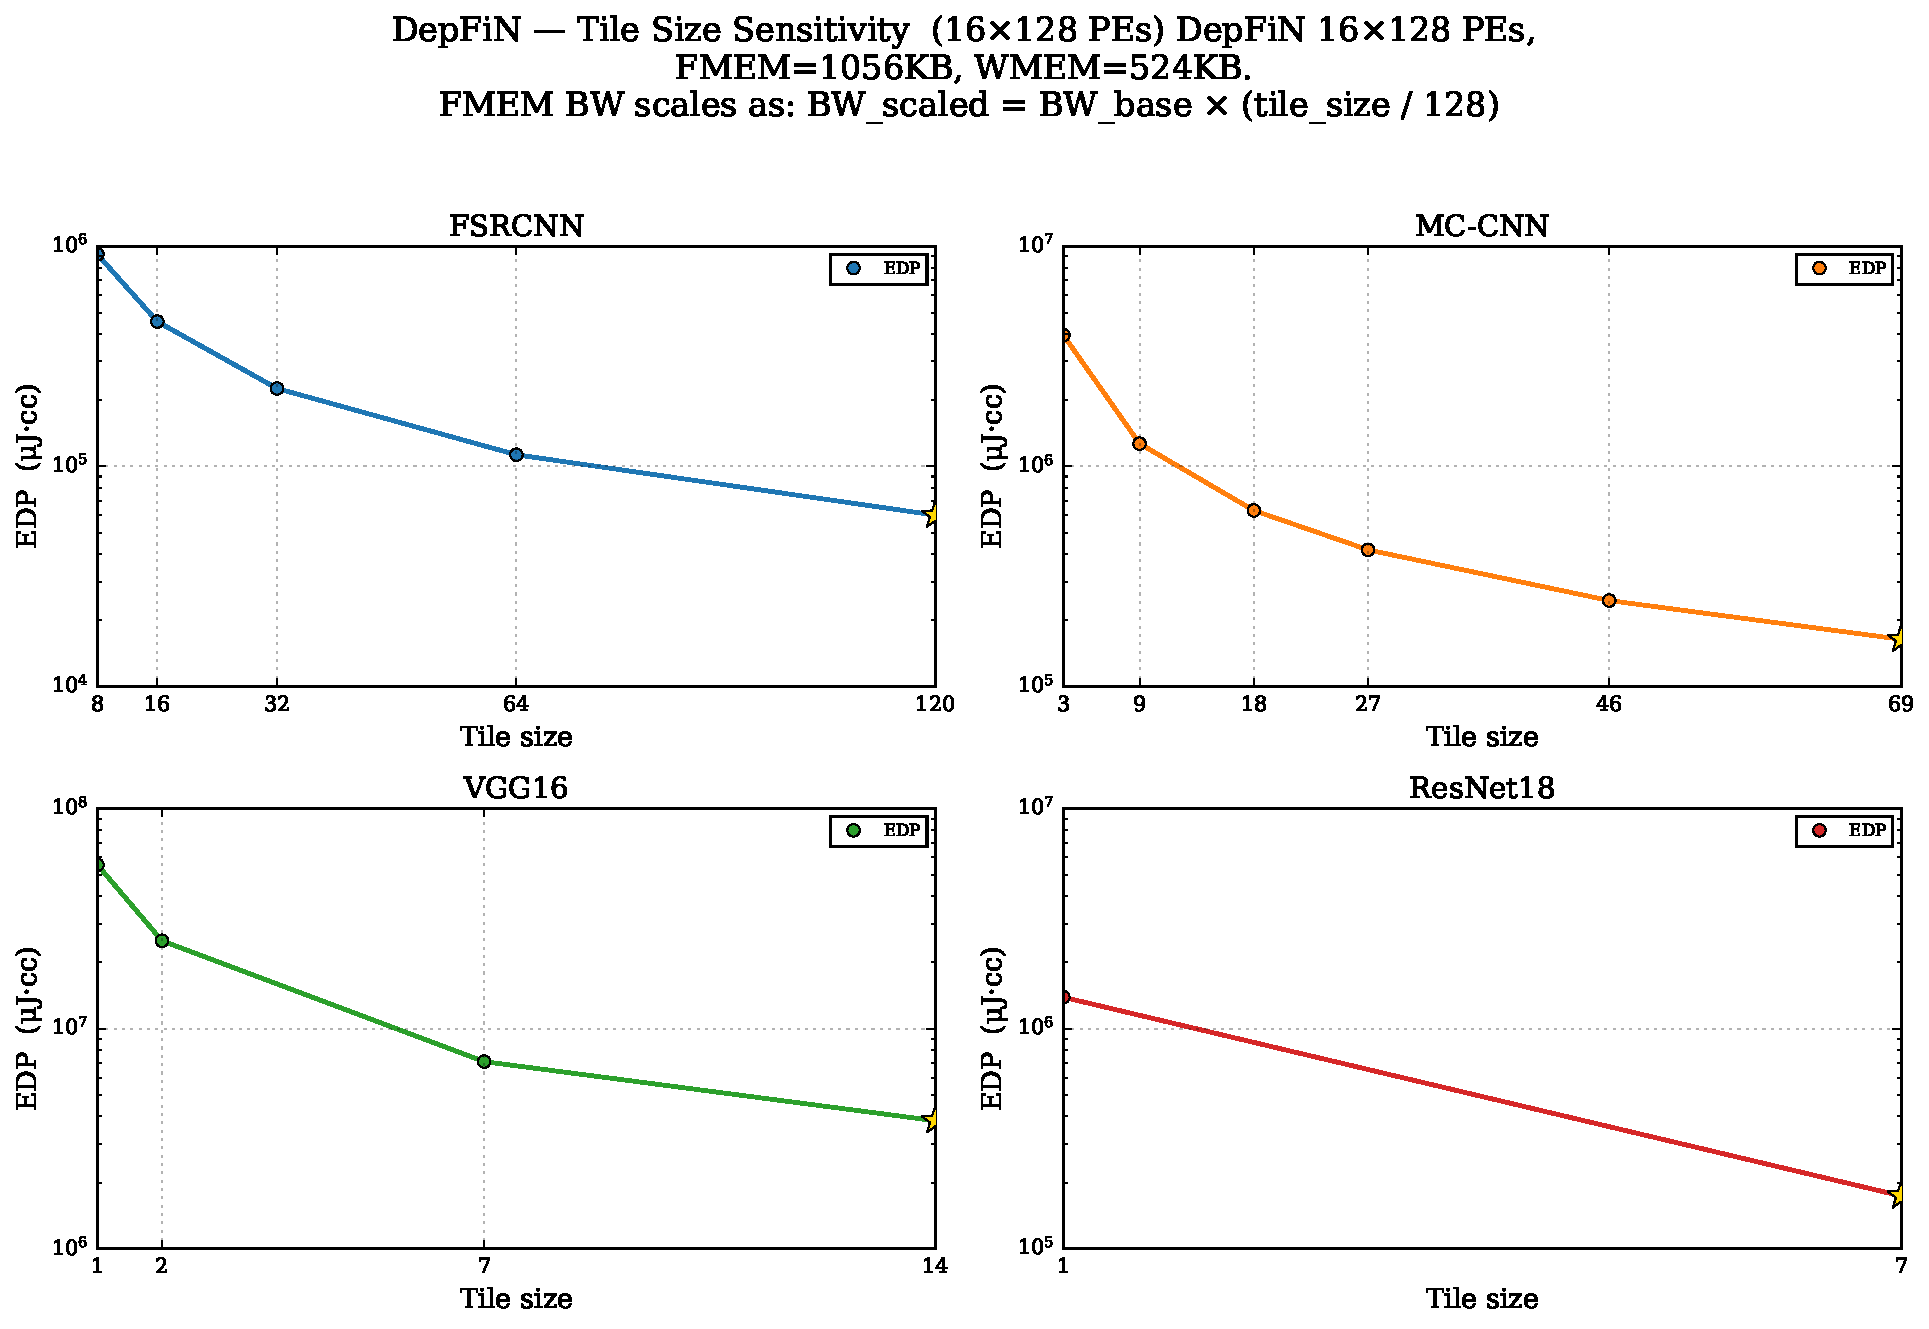
\includegraphics[width=0.85\textwidth]{plots/depfin_cs1_tile_sweep.pdf}
  \caption{DepFiN CS1: EDP vs.\ tile size for each workload
    (FMEM BW scaled with tile).
    The gold star marks the best (minimum-EDP) tile.}
  \label{fig:depfin-cs1}
\end{figure}

\paragraph{FSRCNN (activation-dominant, no stride).}
As a representative example, FSRCNN is swept from tile\,=\,120
(93.8\,\% PE utilization) down to tile\,=\,8 (6.2\,\%).
The EDP degrades by $\approx 15\times$ driven
almost entirely by latency, which increases by $15\times$.
Energy, in contrast, rises by only $+4$\,\%.
The mild energy increase is explained by the weight re-read mechanism:
at tile\,=\,120 the Weight Memory is read $8.1 \times 10^{7}$~times,
whereas at tile\,=\,8 the same weights are re-fetched
$1.2 \times 10^{9}$~times ($15\times$ more), because each of the
additional DRAM passes triggers a full reload of the weight set from Weight Memory.
DRAM reads and writes remain \emph{identical} across all tile sizes,
confirming that the degradation is internal to the on-chip hierarchy.

\paragraph{Weight-dominant workloads.}
VGG16 and ResNet18 exhibit a qualitatively similar trend, but with a
larger energy increase ($+25$\,\% and $+26$\,\% respectively from best
to worst tile), due to larger weight volumes to be reloaded.
The EDP degradation ranges from $8\times$ (ResNet18, tiles 7\,$\to$\,1)
to $15\times$ (VGG16, tiles 14\,$\to$\,1).

\paragraph{Considerations.}

For all four workloads, the largest feasible tile size minimizes EDP in DepFiN.
The dominant effect is latency: smaller tiles force more temporal
iterations at the DRAM level.
The effect of Energy is secondary and grows mainly through increased weight re-reads in the Weight Memory, but this effect is more pronounced for
weight-dominant workloads.